\documentclass[a4paper,14pt]{article} % формат документа

\usepackage{cmap} % поиск в ПДФ
\usepackage[T2A]{fontenc} % кодировка
\usepackage[utf8]{inputenc} % кодировка исходного текста
\usepackage[english,russian]{babel} % локализация и переносы
\usepackage[left = 2cm, right = 1cm, top = 2cm, bottom = 2 cm]{geometry} % поля
\usepackage{listings}
\usepackage{graphicx} % для вставки рисунков
\usepackage{amsmath}
\graphicspath{{pictures/}}
\DeclareGraphicsExtensions{.pdf,.png,.jpg}
\newcommand{\anonsection}[1]{\section*{#1}\addcontentsline{toc}{section}{#1}}

\lstset{ %
	language=Python,                % Язык программирования 
	numbers=left,                   % С какой стороны нумеровать          
	frame=single,                    % Добавить рамку
}

\begin{document}
	\begin{titlepage}

       		\begin{center}
         		\large
		
        			Государственное образовательное учреждение высшего профессионального образования\\
       			“Московский государственный технический университет имени Н.Э.Баумана”
         		\vspace{3cm}
            
            		\textsc{Дисциплина: Анализ алгоритмов}
           		\vspace{0.5cm}
                
            		\textsc{Лабораторная работа № 4}
           		 \vspace{3cm}
            
           		 \LARGE 
		 
		 	Параллельная реализация алгоритма Винограда
           		 \vspace{3cm}
            
            		\begin{flushright}
            			Студент: \\
				Сиденко Анастасия Генадьевна \\   
            			Группа: ИУ7-53Б \\
           			\hfill
            
           			Преподаватели: \\
				Строганов Юрий Владимирович \\
           			Волкова Лилия Леонидовна
            			\vfill
            		\end{flushright}
		
			\large
            		2019 г.
		\end{center}

	\end{titlepage}
    
	\tableofcontents
	
	\newpage
    
	\anonsection{Введение}
	\hfill
	
	Матрицы упоминались ещё в древнем Китае, называясь тогда «волшебным квадратом». Основным применением матриц было решение линейных уравнений. Также волшебные квадраты были известны чуть позднее у арабских математиков, примерно тогда появился принцип сложения матриц. Сама теория матриц начала своё существование в середине XIX века. Термин «матрица» ввел Джеймс Сильвестр в 1850 г. Сегодня матрицы применяются уже не только при решении линейных уравнений. [1]
	
	Умножение матриц — это один из базовых алгоритмов, который широко применяется в различных численных методах, и в частности в алгоритмах машинного обучения. Многие реализации прямого и обратного распространения сигнала в сверточных слоях нейронной сети базируются на этой операции. [2] В физике и других прикладных науках матрицы – являются средством записи данных и их преобразования.[4] В программировании – в написании программ, массивы. Широкое применение в компьютерной графике: любая картинка на экране – это двумерная матрица, элементами которой являются цвета точек, а также матрицы используются для преобразования фигур. [5]
	
	В психологии понимание термина сходно с данным термином в математике, но взамен математических объектов подразумеваются некие "психологические объекты" – например, тесты. [6]
	
	Кроме того, умножение матриц имеет широкое применение в экономике[7], биологии[8], химии[9]. 
	
	Также существует абстрактная модель – теорию бракосочетаний в первобытном обществе, где с помощью матриц были показаны разрешенные варианты браков для представителей и даже потомков того или иного племени.[3]
	
	Таким образом, умножение матриц -- широко используемая операция, а значит существует необходимость сокращения вычислений данной операции. 
	
	\hfill
	
	В данной лабораторной работе ставятся следующие задачи. 
        \begin{enumerate} 
		\item Изучение алгоритма Винограда с оптимизациями и его распараллеливание. 
		\item Оценка трудоемкости алгоритма умножения матриц.
		\item Получение практических навыков параллельной реализации данного алгоритма на одном из языков программирования (с нативными потоками). 
		\item Сравнительный анализ алгоритма по затрачиваемым ресурсам (зависимость времени от длины строки) для разного количества потоков. 
		\item Экспериментальное подтверждение различий в трудоемкости алгоритма. 
	\end{enumerate}
	
	\newpage


        \section{Аналитическая часть}
        \hfill
        
        Умножение матриц – это одна из основных вычислительных операций. Вычислительная сложность стандартного алгоритма умножения матриц порядка N составляет $O(N^3)$. Но существуют более сложные алгоритмы, которые дают лучший результат, например алгоритм Винограда. 
        
        
        \subsection{Описание задачи}
        \hfill
        
	Пусть даны две прямоугольные матрицы $A[M \times N]$ и $B[N \times Q]$:
	$$
	A = 
  	\begin{bmatrix} 
   		a_{11} & a_{12} & \cdots & a_{1n} \\
    		a_{21} & a_{22} & \cdots & a_{2n} \\ 
   		\vdots & \vdots & \ddots & \vdots \\ 
		a_{m1} & a_{m2} & \cdots & a_{mn}
	\end{bmatrix}
	B =   
	\begin{bmatrix} 
		b_{11} & b_{12} & \cdots & b_{1q} \\
		b_{21} & b_{22} & \cdots & b_{2q} \\ 
		\vdots & \vdots & \ddots & \vdots \\ 
    		b_{n1} & b_{n2} & \cdots & b_{nq}
  	\end{bmatrix}
	$$
	Тогда матрица $C[M \times Q]$ -- произведение матриц:
	$$
	C = 
	\begin{bmatrix} 
    		c_{11} & c_{12} & \cdots & c_{1q} \\
   		c_{21} & c_{22} & \cdots & c_{2q} \\ 
   		\vdots & \vdots & \ddots & \vdots \\ 
    		c_{m1} & c_{m2} & \cdots & c_{mq}
  	\end{bmatrix},
	$$
	в которой каждый элемент вычисляется по формуле 1: 
	$$c_{ij} = \sum_{k=1}^n a_{ik}b_{kj}, ~(i=1, 2, \ldots l;j=1, 2, \ldots n)~~(1)$$
	
	Операция умножения двух матриц выполнима только в том случае, если число столбцов в первом сомножителе равно числу строк во втором; в этом случае говорят, что матрицы ''согласованы''.
	
	В данной лабораторной работе стоит задача распараллеливания алгоритма Винограда. Так как каждый элемент матрицы С вычисляется независимо от других и матрицы А и В не изменяются, то для того, чтобы вычислить произведение параллельно, достаточно просто указать какие элементы С какому потоку вычислять.
	
	Теоретически, для нахождения значения каждой из ячеек можно создать свой поток. Но ОС не позволит создать такое число потоков, ресурсов на их создание не хватит и создание потока также занимает определенный промежуток времени.
	
	Оптимальное число потоков равно $4*\text{количество логических ядер}$.
	
	В данной работе для реализации многопоточности будут использованы нативные потоки. В программировании нативные потоки -- это потоки выполнения, управляющиеся операционной системой в пространстве ядра.[10]
	
	Помимо нативных, существуют зелёные потоки -- это потоки выполнения, управление которыми вместо операционной системы выполняет виртуальная машина. Управление ими происходит в пользовательском пространстве, что позволяет им работать в условиях отсутствия поддержки встроенных потоков.[10]
        	
        \subsection{Пути решения}
        \hfill
        
        Сложность вычисления произведения матриц порядка N по определению составляет составляет $O(N^3)$, однако существуют более эффективные алгоритмы, применяющиеся для перемножения матриц. 
        
	Также можно распараллелить данные алгоритмы, скорость работы, при разумном выборе количеств потоков, возрастет. 
	                
        \subsection{Выводы} 
        \hfill
        
        В данной работе стоит задача реализации алгоритма умножения матриц. Необходимо сравнить обычную реализацию алгоритма с многопоточной. 
           

	\newpage

	\section{Конструкторская часть}
	\hfill
	
	 В данной работе для нахождения произведения матриц используется алгоритм Винограда и его многопоточная реализация.
	 
	Распределять нагрузку будем простым способом: каждый из потоков обрабатывает одинаковое число рядов и один поток ещё обрабатывает остаток.  
	
	\subsection{Функциональная модель}
	На рисунке 1 представлена функциональная модель нашей задачи.  
	\begin{center}
		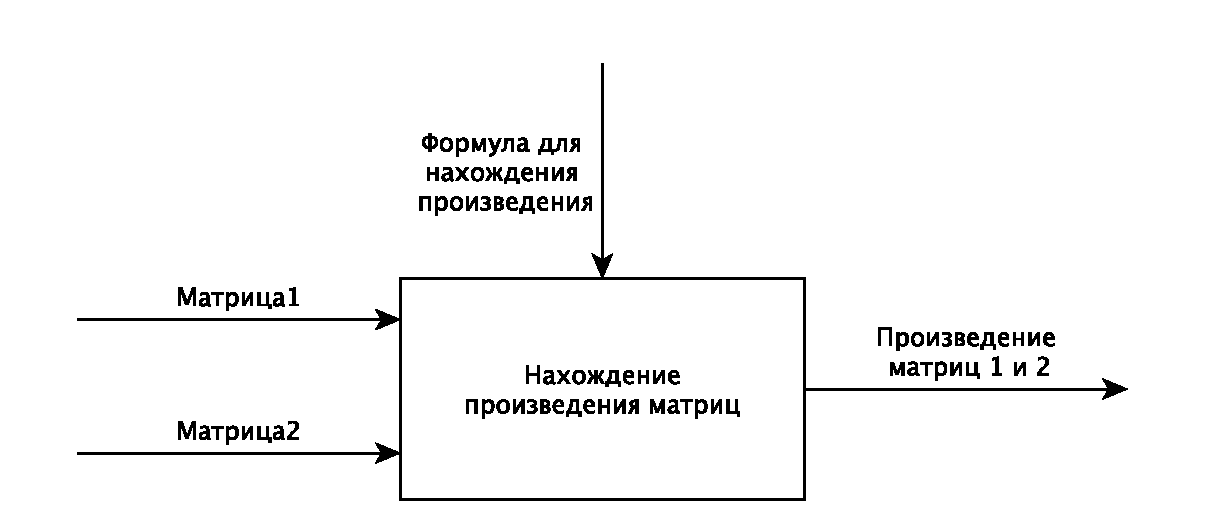
\includegraphics[scale = 0.8]{idef0} \\ Рис.  1 - Функциональная модель алгоритма нахождения произведения матриц. 
	\end{center}
	
        
        \subsection{Схемы алгоритмов}
        \hfill
        
        Приведем схему алгоритма (см. рисунки 2-3). 
        
        \hfill

	\hfill
	\paragraph{Алгоритм Винограда с оптимизациями}
	
	\begin{center}
        		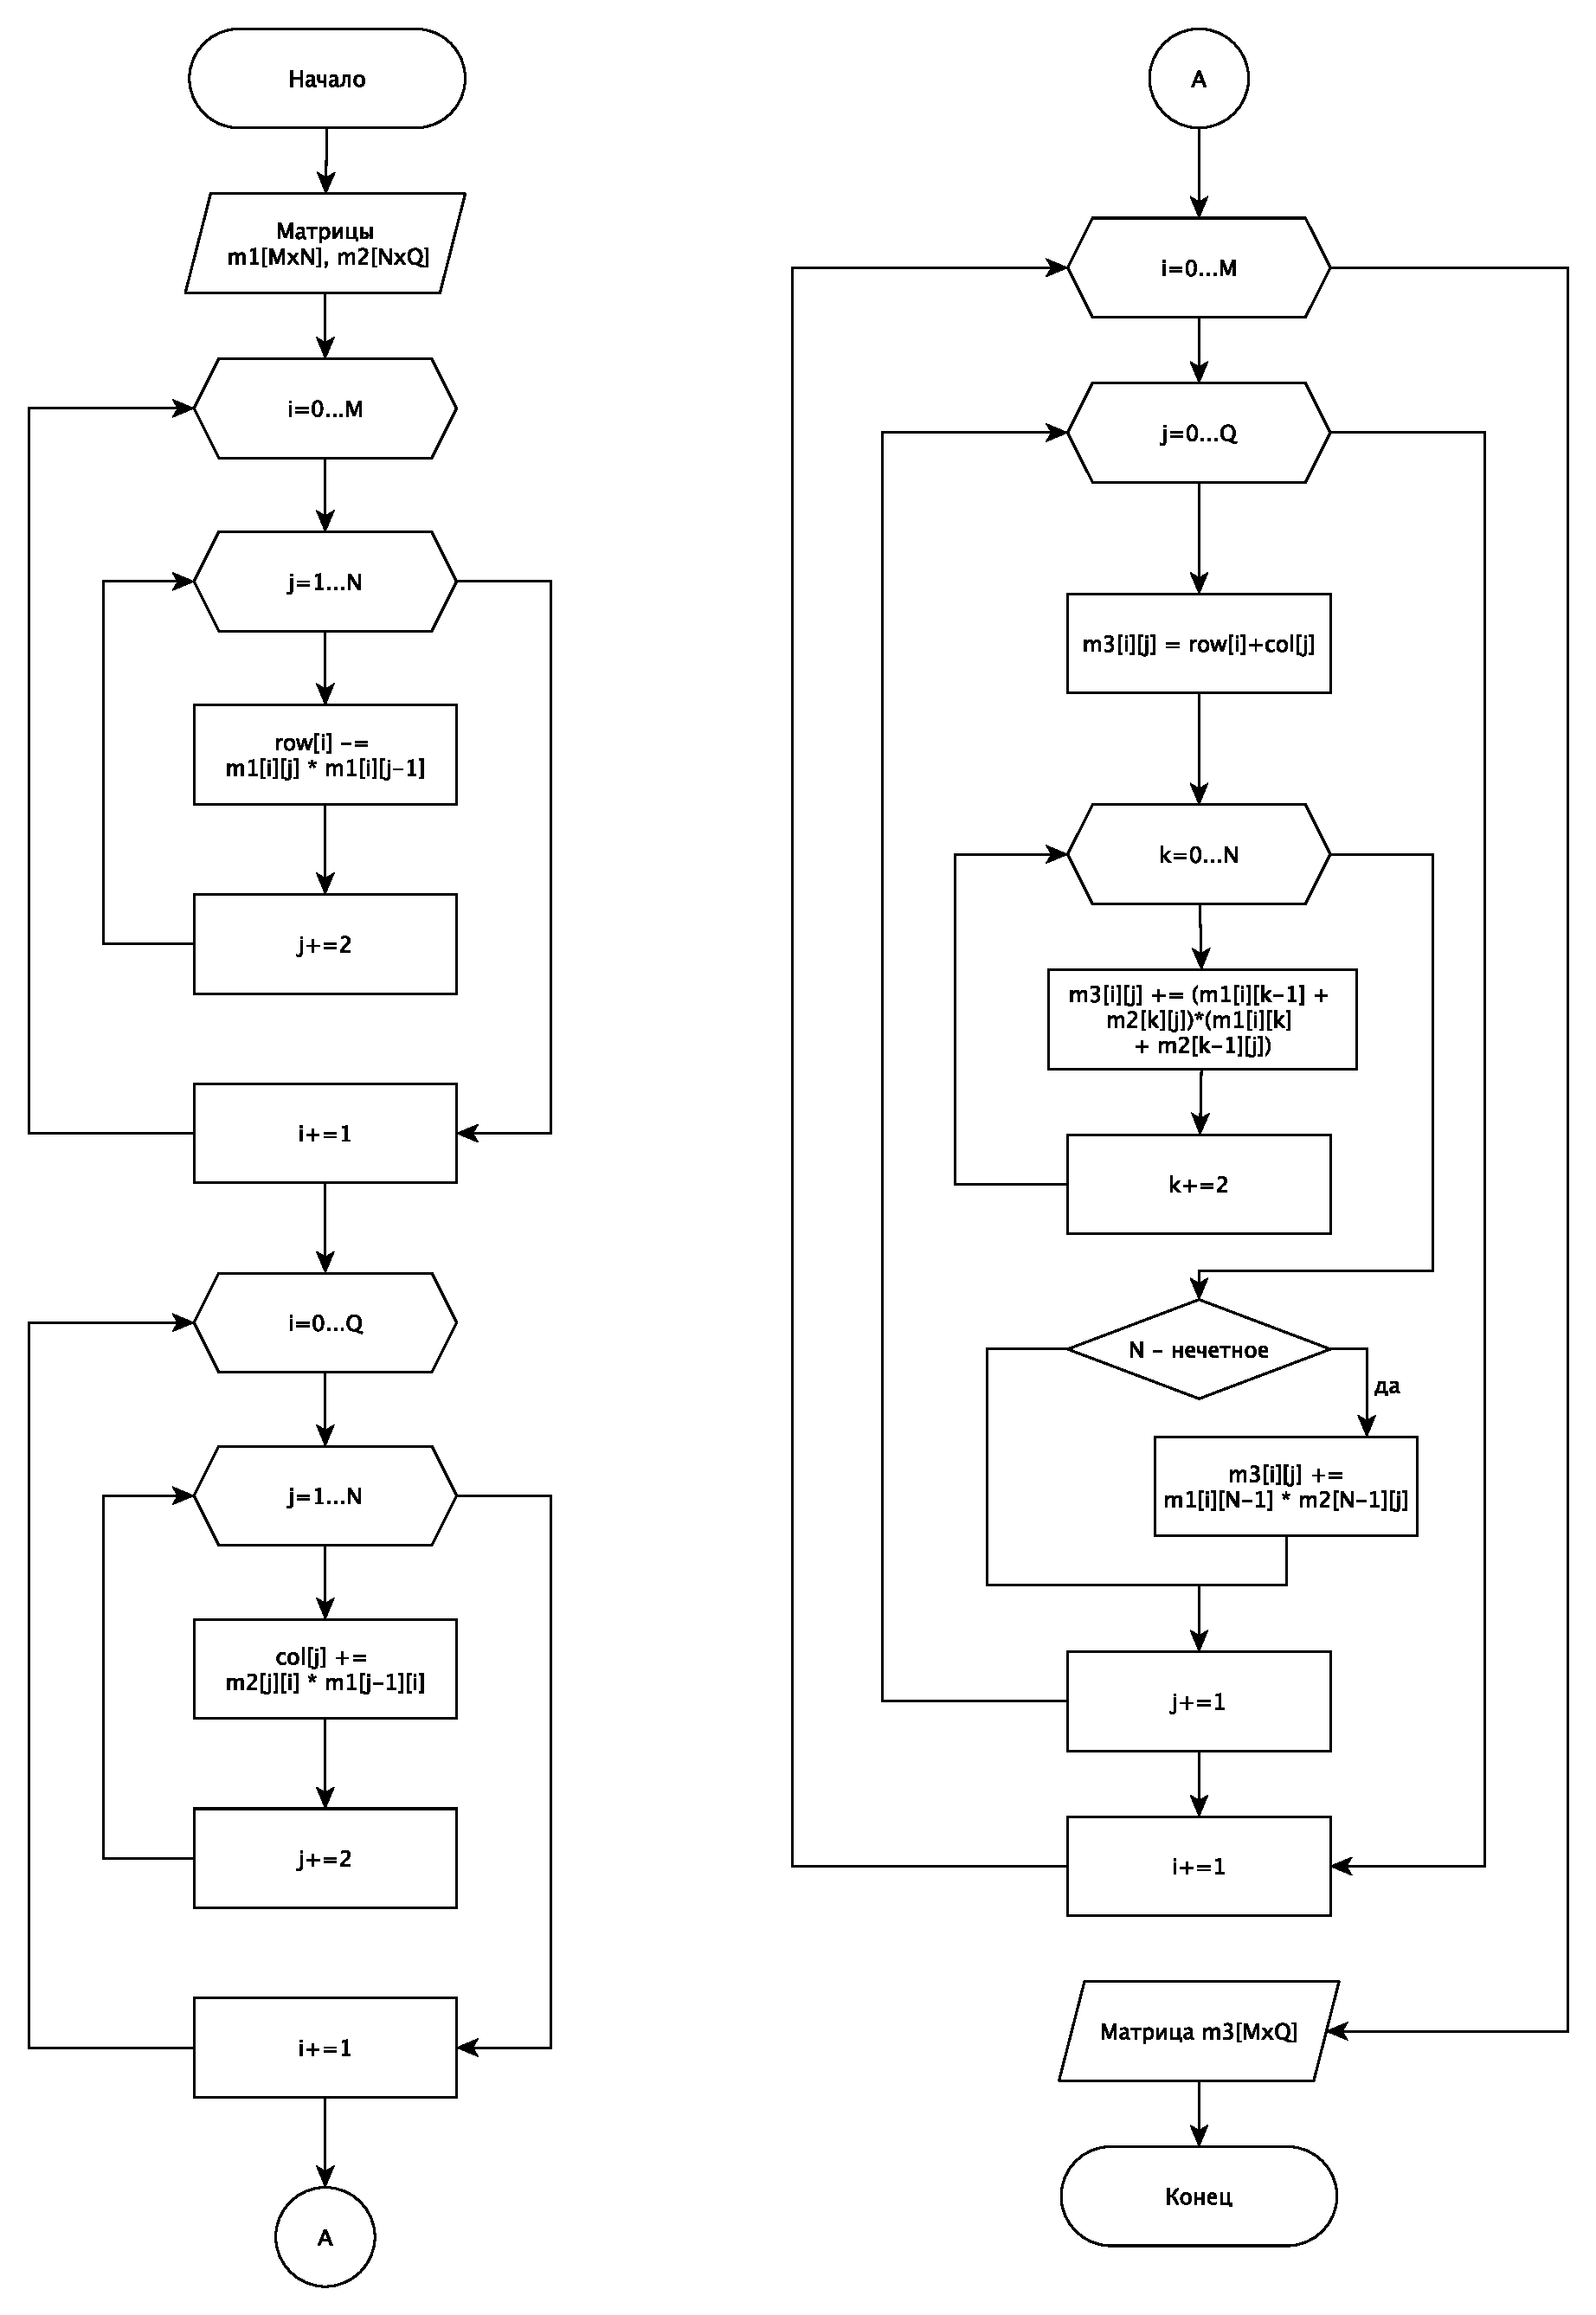
\includegraphics[scale = 0.53]{shema1} \\ Рис. 2 - Алгоритм нахождения произведения матриц методом Винограда с оптимизациями
	\end{center}
	
	\paragraph{Многопоточный алгоритм Винограда с оптимизациями}
	
	\begin{center}
        		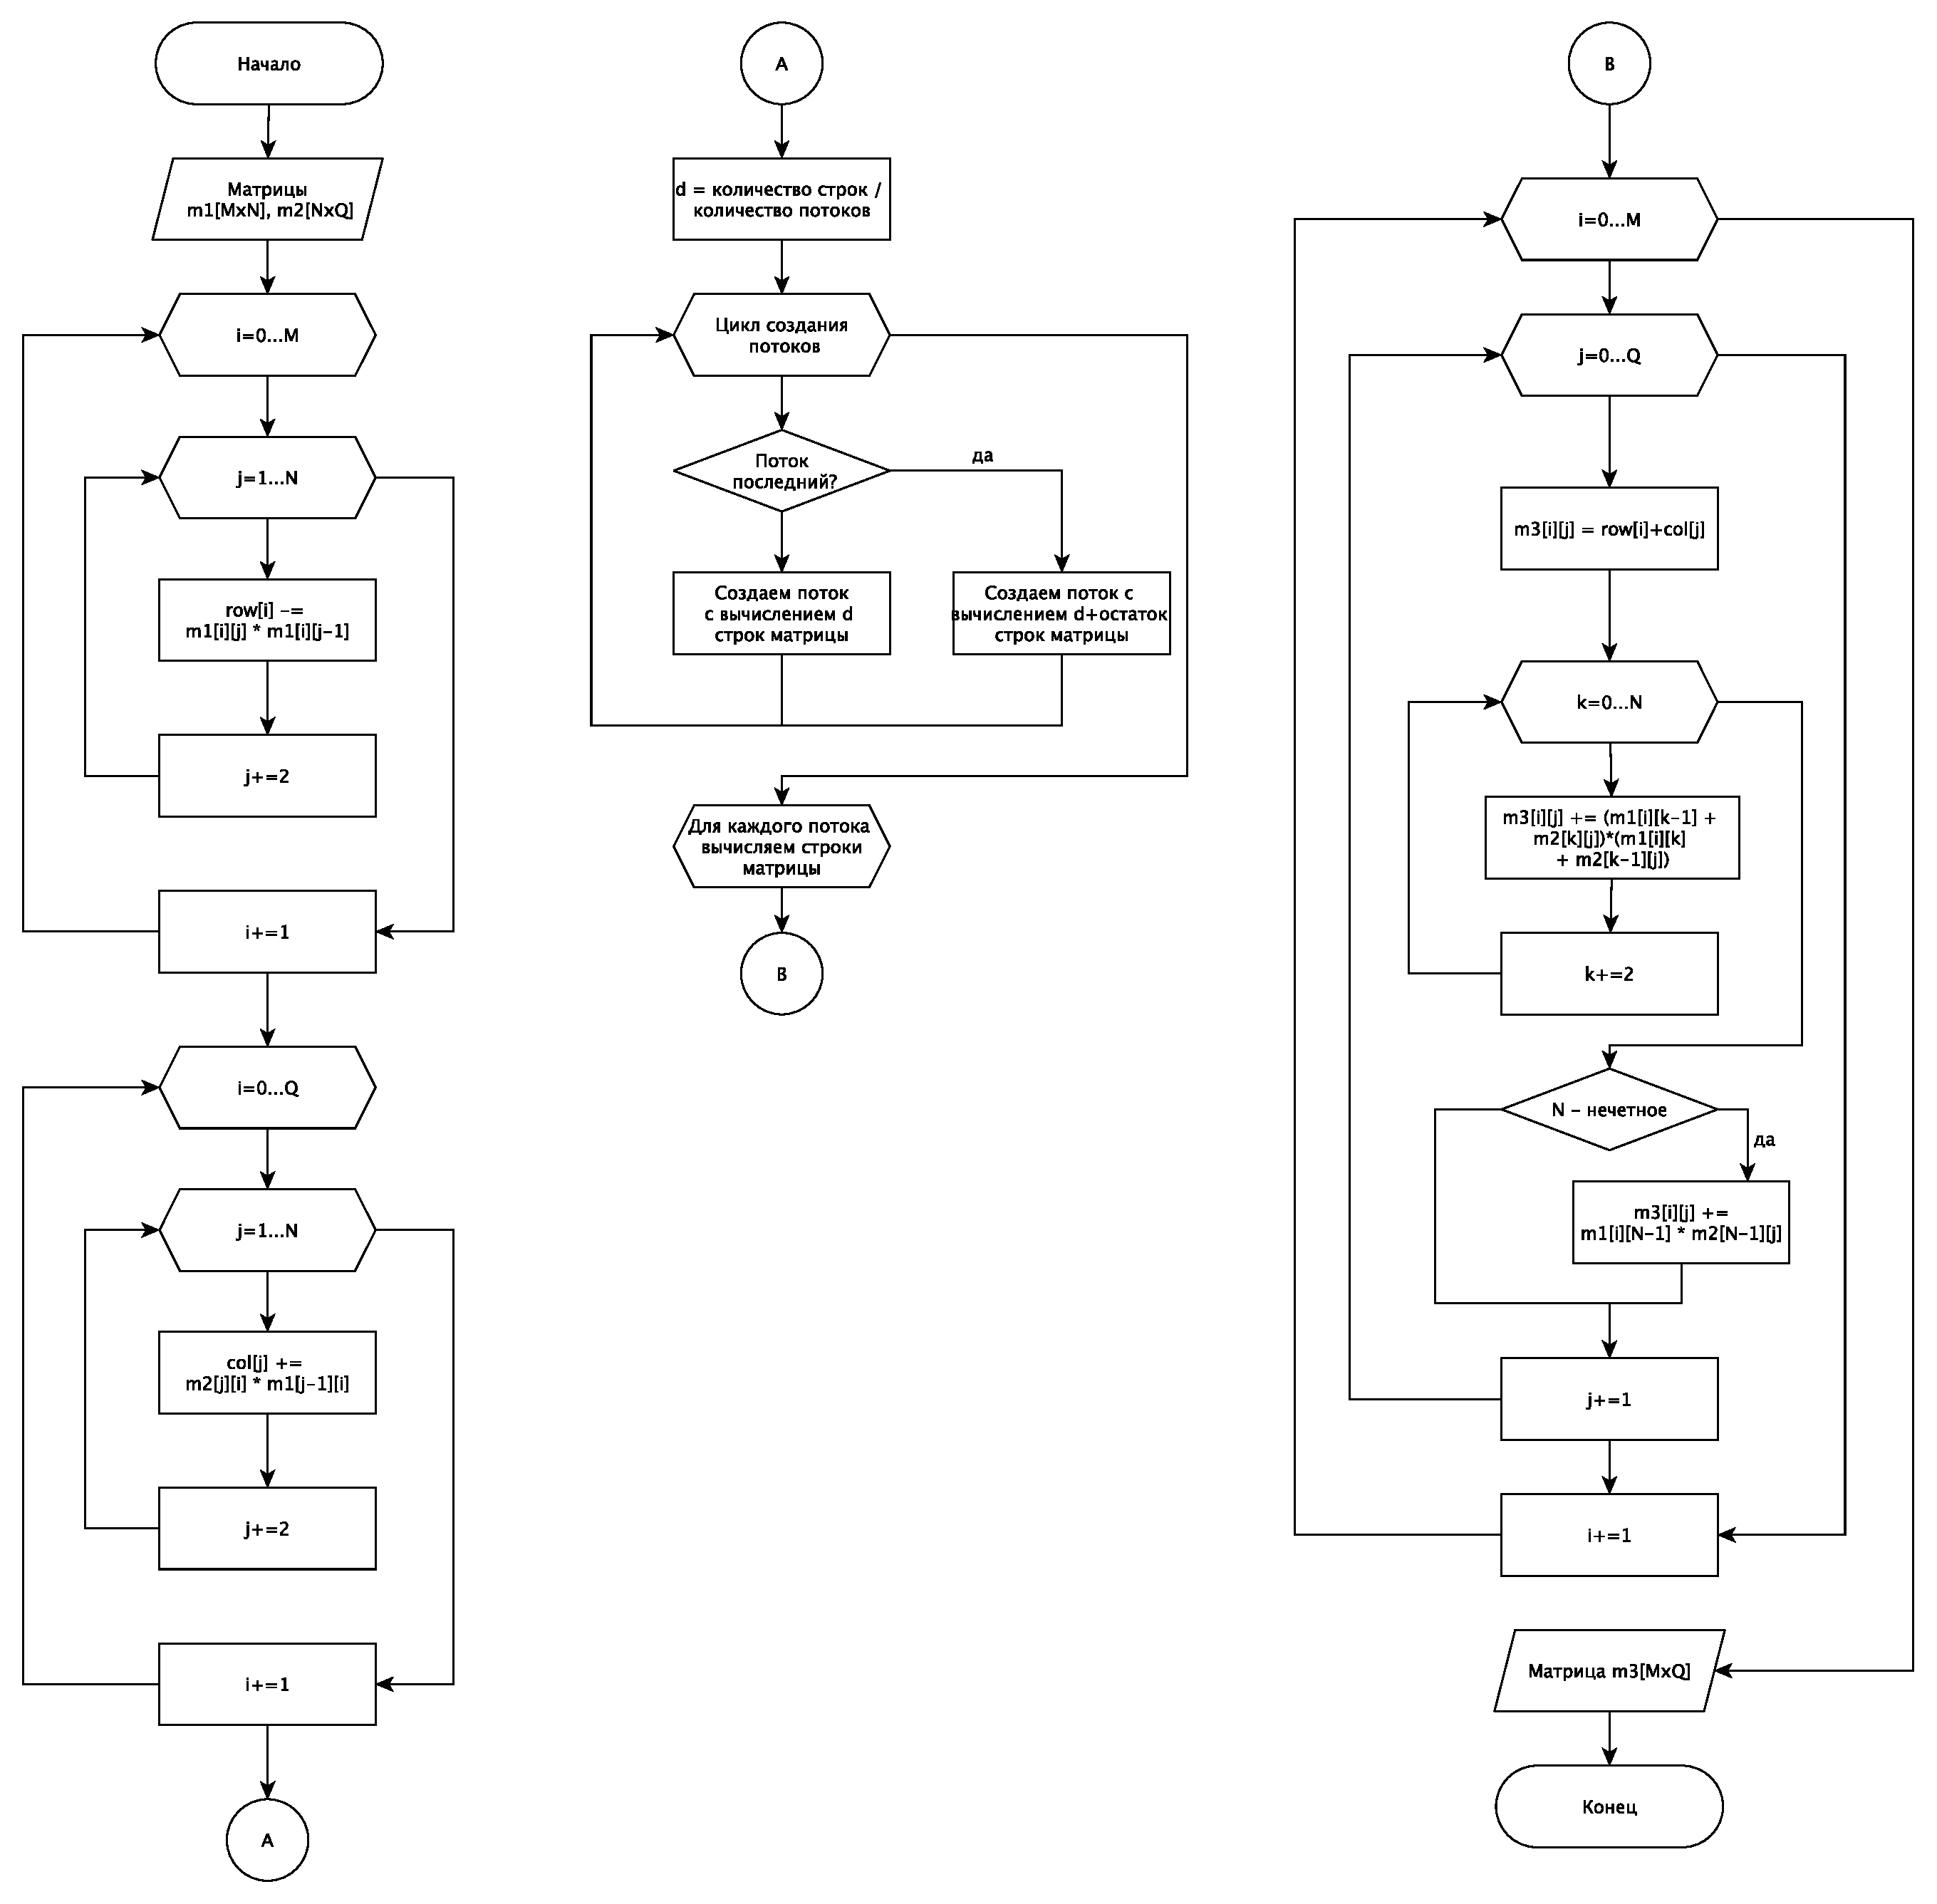
\includegraphics[scale = 0.4]{shema2} \\ Рис. 3 - Алгоритм нахождения произведения матриц методом Винограда с оптимизациями и параллельными вычислениями
	\end{center}
	
	\hfill
	
	\subsection{Выводы}
	\hfill
	
	Несмотря на сложность увеличение сложности реализации алгоритма Винограда с параллельными потоками, скорость вычисления произведения должна значительно сократиться. 
	
	Необходимо разработать данные алгоритмы и убедиться в корректности наших предположений. 
	
    	\newpage

        \section{Технологическая часть}
        \hfill
        
        Стоит задача разработки и сравнительного анализа алгоритмов, вычисляющих произведения матриц в однопоточной и многопоточной реализациях. 
        \hfill
        
        В реализациях в целях увеличения точности подсчета времени вывод матрицы был вынесен за пределы функций-алгоритмов. В целях наглядности были опущены части программ, не относящиеся к работе алгоритмов.
        
        \hfill

        \subsection{Требования к программному обеспечению}
        \hfill
        
        ПО должно предоставлять возможность замеров процессорного времени выполнения реализации каждого алгоритма. Требуется провести замеры для варьирующихся размеров матриц: от 100 до 1000 и от 101 до 1001. Один эксперимент ставится не менее 5 раз, результат одного эксперимента рассчитывается как среднее значение результатов проведенных испытаний с одинаковыми входными данными.
        \hfill
        
        \subsection{Средства реализации}
        \hfill
        
        В качестве языка программирования был выбран С++, так как я знакома с этих языком программирования и он удовлетворяет требованиям об необходимости использовании нативных потоков. [11]
        \hfill
        
        Для замеров времени была выбран метод $high\_resolution\_clock::now()$, возвращает текущее время процессора как число тиков, выраженное в микросекундах в Unix.
        \hfill
        
        Для генерации случайных матриц, заданного размера использовался метод $rand()$. 
        
        Для работы с потоками использована библиотека $<thread>$. 
        \hfill
        
        \subsection{Листинг кода}
        \hfill
        
        	\textbf{Многопоточный алгоритм Винограда:}
          
	\begin{lstlisting}
void cycle(vector< vector<int> > m1, vector< vector<int> > m2, 
		vector< vector<int> > &m3, vector<int> row, vector<int> col, 
		int m_begin, int m_end) {
int n = m1[0].size();
int q = m2[0].size();
for (int i = m_begin; i < m_end; i++) {
   for (int j = 0; j < q; j++){
      m3[i][j] = row[i] + col[j];
      for (int k = 1; k < n; k += 2) {
         m3[i][j] += (m1[i][k - 1] + m2[k][j])*(m1[i][k] + m2[k - 1][j]);
      }
      if (1 == n % 2)
         m3[i][j] += m1[i][n - 1] * m2[n - 1][j];
      }
}
}

int vinograd_optimizate_multiplication_matrix(vector< vector<int> > m1, 
			vector< vector<int> > m2, int count) {
   if (m2.size() != m1[0].size()) {
      return -1;
   } else {
      int m = m1.size();
      int n = m1[0].size();
      int q = m2[0].size();
      vector< vector<int> > m3(m, vector<int> (q, 0));

      vector<int> row(m, 0);
      for (int i = 0; i < m; i++) {
         for (int j = 1; j < n; j += 2){
            row[i] -= m1[i][j] * m1[i][j - 1];
         }
      }

      vector<int> col(q, 0);
      for (int j = 0; j < q; j++) {
         for (int i = 1; i < n; i += 2){
            col[j] -= m2[i][j] * m2[i - 1][j];
         }
      }

      int d = m / count;
      vector<thread> func_thread;
      for (int i = 0; i < count; i++) {
         if (i == count - 1) {
            func_thread.push_back(thread(cycle, m1, m2, ref(m3), row, col, 
            					i * d, (1 + i) * d + m % count));
         } else {
            func_thread.push_back(thread(cycle, m1, m2, ref(m3), row, col, 
            					i * d, (1 + i) * d));
         }
      }
       for (int i = 0; i < count; i++) {
          func_thread[i].join();
       }
   }
}
	\end{lstlisting}

	\textbf{Алгоримт Винограда: }
	\begin{lstlisting}

int vinograd_optimizate_multiplication_matrix(vector< vector<int> > m1, 
			vector< vector<int> > m2, int count) {
   if (m2.size() != m1[0].size()) {
      return -1;
   } else {
      int m = m1.size();
      int n = m1[0].size();
      int q = m2[0].size();
      vector< vector<int> > m3(m, vector<int> (q, 0));

      vector<int> row(m, 0);
      for (int i = 0; i < m; i++) {
         for (int j = 1; j < n; j += 2){
            row[i] -= m1[i][j] * m1[i][j - 1];
         }
      }

      vector<int> col(q, 0);
      for (int j = 0; j < q; j++) {
         for (int i = 1; i < n; i += 2){
            col[j] -= m2[i][j] * m2[i - 1][j];
         }
      }

      for (int i = m_begin; i < m_end; i++) {
         for (int j = 0; j < q; j++){
            m3[i][j] = row[i] + col[j];
            for (int k = 1; k < n; k += 2) {
               m3[i][j] += (m1[i][k - 1] + m2[k][j])*(m1[i][k] + m2[k - 1][j]);
            }
            if (1 == n % 2)
               m3[i][j] += m1[i][n - 1] * m2[n - 1][j];
         }
      }
   }
}
	\end{lstlisting}

        
	\subsection{Тестирование}
	\hfill
	
	В таблице 1 представлена заготовка данных для тестирования наших алгоритмов. 
	\begin{center}
		\begin{tabular}{  | c | c | c | }
			\hline
			\textbf{Матрица1} & \textbf{Матрица2} & \textbf{Ожидаемый результат} \\ \hline
			$\begin{bmatrix} 
   			1&2&3 \\
    			4&5&6 \\ 
   			7&8&9 \\ 
			\end{bmatrix}$ & 
			$\begin{bmatrix} 
   			1&2&3 \\
    			4&5&6 \\ 
   			7&8&9 \\ 
			\end{bmatrix}$ &
			$\begin{bmatrix} 
   			30&36&42 \\
    			66&81&96 \\ 
   			102&126&150 \\ 
			\end{bmatrix} $ \\ \hline
			
			$\begin{bmatrix} 
   			1&2&3 \\
    			4&5&6 \\ 
   			7&8&9 \\ 
			\end{bmatrix}$ & 
			$\begin{bmatrix} 
   			1&2&3 \\
    			4&5&6 \\ 
			\end{bmatrix}$ &
			$\text{Матрицы не могут быть перемножены}$ \\ \hline
			
			$\begin{bmatrix} 
   			1&2 \\
    			4&5 \\ 
   			7&8 \\ 
			\end{bmatrix}$ & 
			$\begin{bmatrix} 
   			1&2&3 \\
    			4&5&6 \\ 
			\end{bmatrix}$ &
			$\begin{bmatrix} 
   			9&12&15 \\
    			24&33&42 \\ 
   			39&54&69 \\ 
			\end{bmatrix} $ \\ \hline
		\end{tabular}
		
		\hfill
		
		Таблица 1.
		Подготовленные тестовые данные.  
	\end{center}
	
	\subsection{Выводы}
	\hfill
	
	Реализованы алгоритмы, подготовлены тесты для оценки качества их работы. 
        
        Получены практические навыки реализации алгоритмов матричного умножения методом Винограда и его распараллеливание. 
	
        \hfill
        
        
        \newpage

        \section{Экспериментальная часть}
       
        Оценка качества работы алгоритмов. Экспериментальное сравнение работы различных алгоритмов (зависимость времени выполнения от размерности матрицы). 
        \subsection{Примеры работы}
	\hfill
	
	На рисунке 4 представлены примеры работы программы на разных входных данных. В параметрах командной строки можно указать желаемое число используемых потоков, по умолчанию 1.
	\begin{figure}[ht]\center
		\begin{tabular}{cc}
			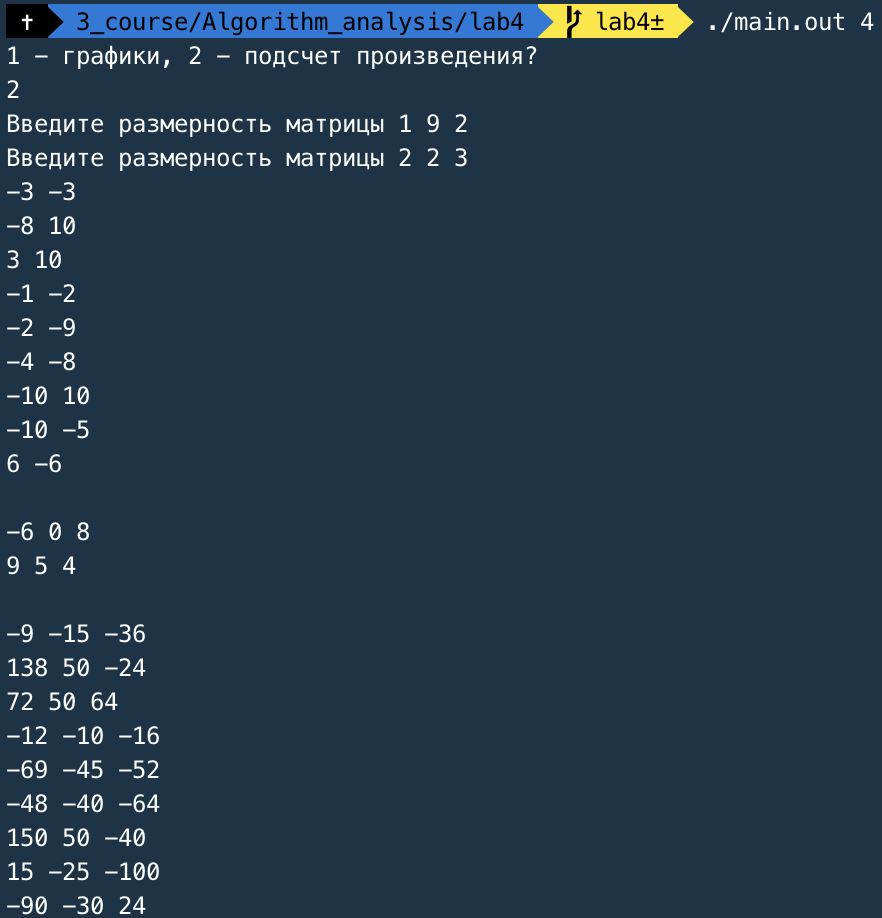
\includegraphics[width=80mm]{ex1} & 
\includegraphics[width=80mm]{ex2} \\
			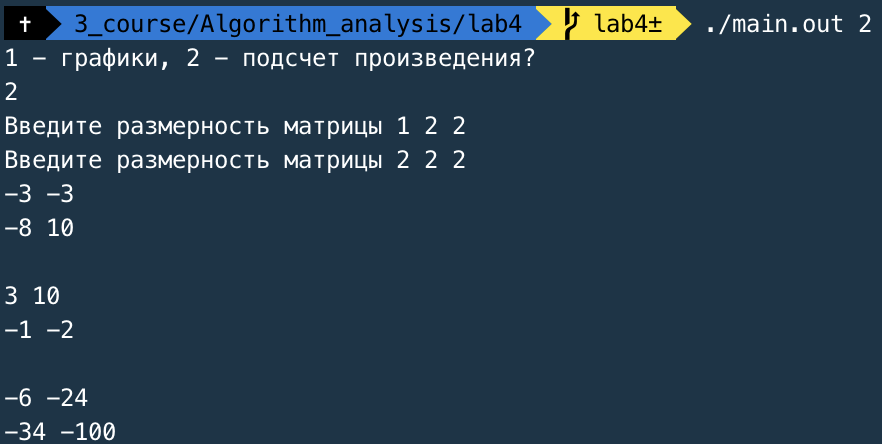
\includegraphics[width=80mm]{ex3} & 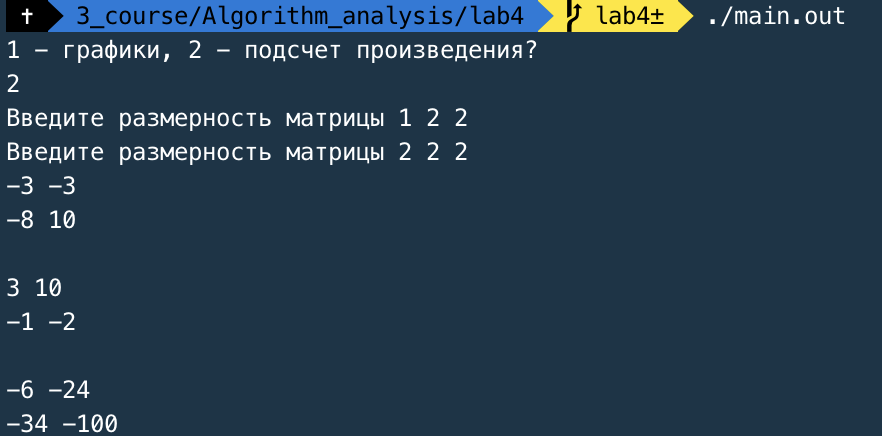
\includegraphics[width=80mm]{ex4} \\
			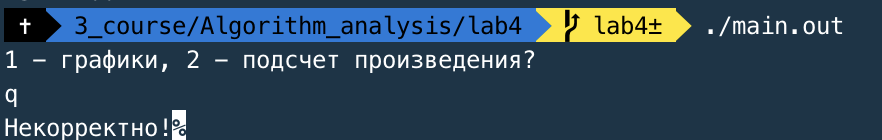
\includegraphics[width=80mm]{ex5} & 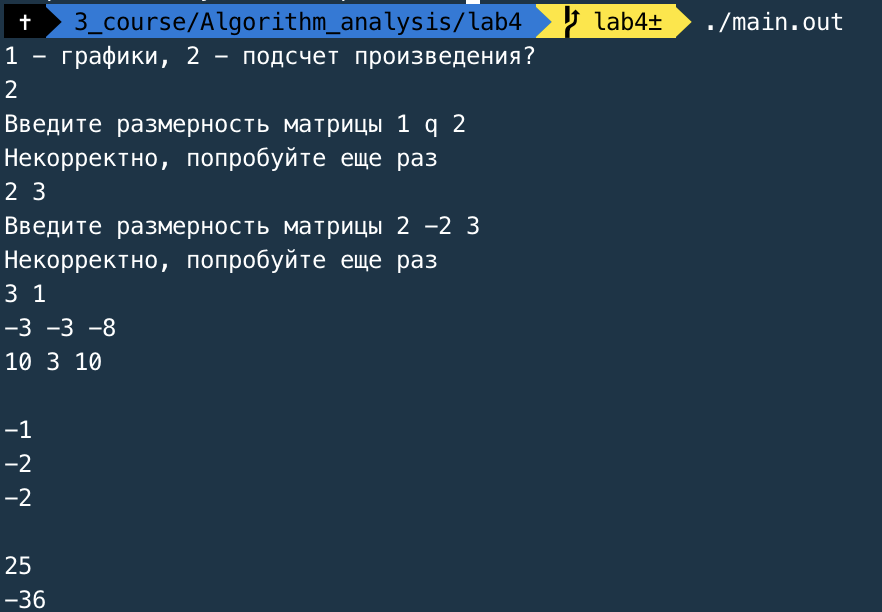
\includegraphics[width=80mm]{ex6}
		\end{tabular}
		\\ Рис. 4 - Примеры работы
	\end{figure}
	        
        \subsection{Результаты тестирования}
        
	\hfill
	Проверяем нашу программу на тестах из таблицы 1. Полученные результаты представлены в таблице 2. 
	\begin{center}
		\begin{tabular}{ | c | c | c | c | c |}
			\hline
			\textbf{Матрица1} & \textbf{Матрица2} & \textbf{Виноград} \\ \hline
			$\begin{bmatrix} 
   			1&2&3 \\
    			4&5&6 \\ 
   			7&8&9 \\ 
			\end{bmatrix}$ & 
			$\begin{bmatrix} 
   			1&2&3 \\
    			4&5&6 \\ 
   			7&8&9 \\ 
			\end{bmatrix}$ &
			$\begin{bmatrix} 
   			30&36&42 \\
    			66&81&96 \\ 
   			102&126&150 \\ 
			\end{bmatrix} $ \\ \hline
			
			$\begin{bmatrix} 
   			1&2&3 \\
    			4&5&6 \\ 
   			7&8&9 \\ 
			\end{bmatrix}$ & 
			$\begin{bmatrix} 
   			1&2&3 \\
    			4&5&6 \\ 
			\end{bmatrix}$ &
			$\begin{matrix} 
   			\text{Матрицы не могут} \\
    			\text{быть перемножены}\\ 
			\end{matrix} $ \\ \hline
			
			$\begin{bmatrix} 
   			1&2 \\
    			4&5 \\ 
   			7&8 \\ 
			\end{bmatrix}$ & 
			$\begin{bmatrix} 
   			1&2&3 \\
    			4&5&6 \\ 
			\end{bmatrix}$ &
			$\begin{bmatrix} 
   			9&12&15 \\
    			24&33&42 \\ 
   			39&54&69 \\ 
			\end{bmatrix} $ \\ \hline
		\end{tabular}
		
		\hfill
		
		Таблица 2.
		Тестирование программы.  
	\end{center}
	
	
	\textbf{Тесты пройдены}

	\subsection{Замеры времени}
	\hfill
	
	На графиках 5-6 представлено сравнение алгоритмов умножения матриц. 
	\begin{center}
        		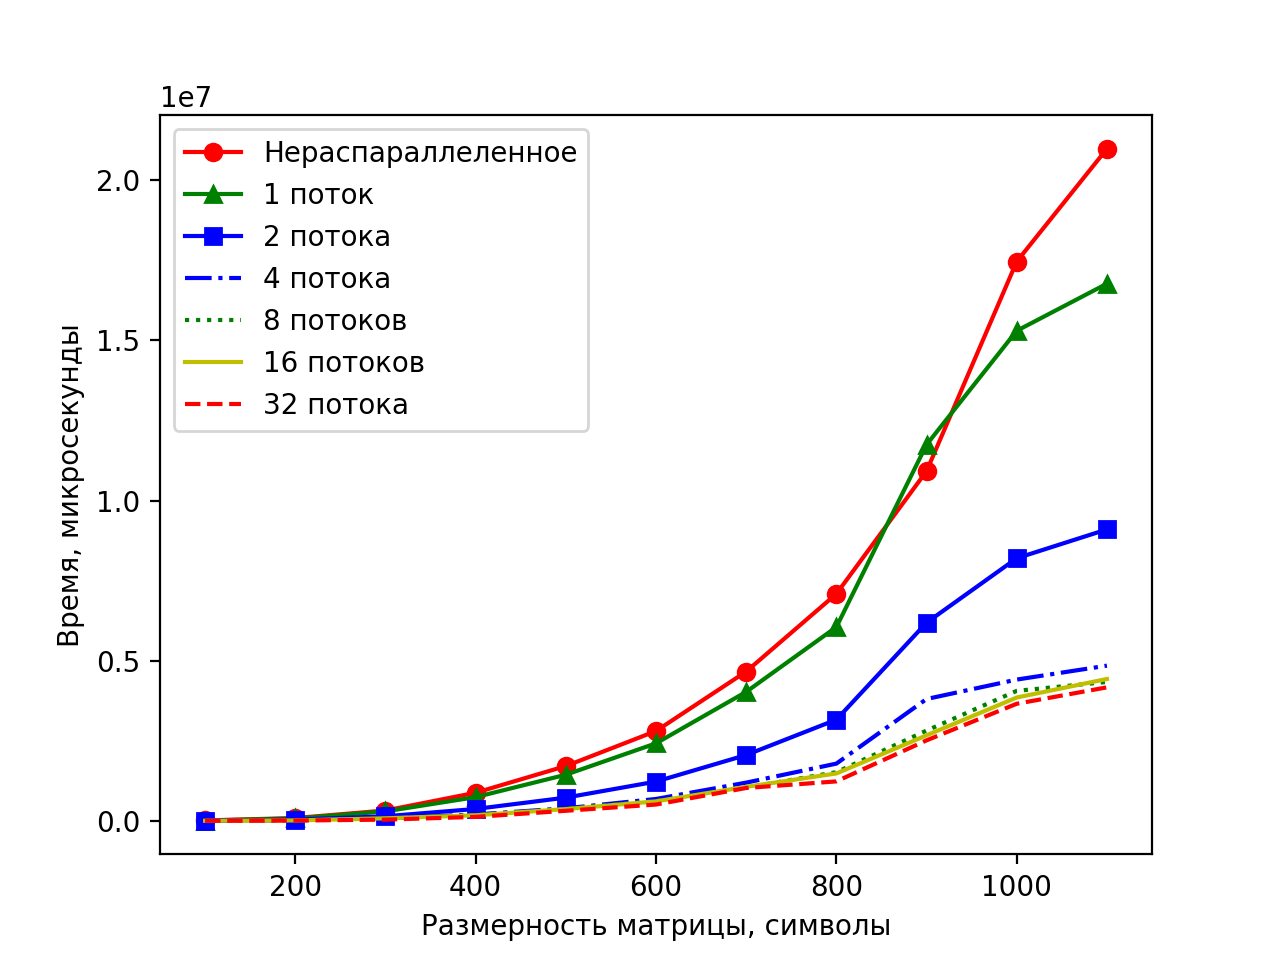
\includegraphics[scale = 1]{graph1} \\ Рис. 6 - Сравнение реализации алгоритмов нахождения произведения матриц при четных размерностях
	\end{center}
	
	\begin{center}
        		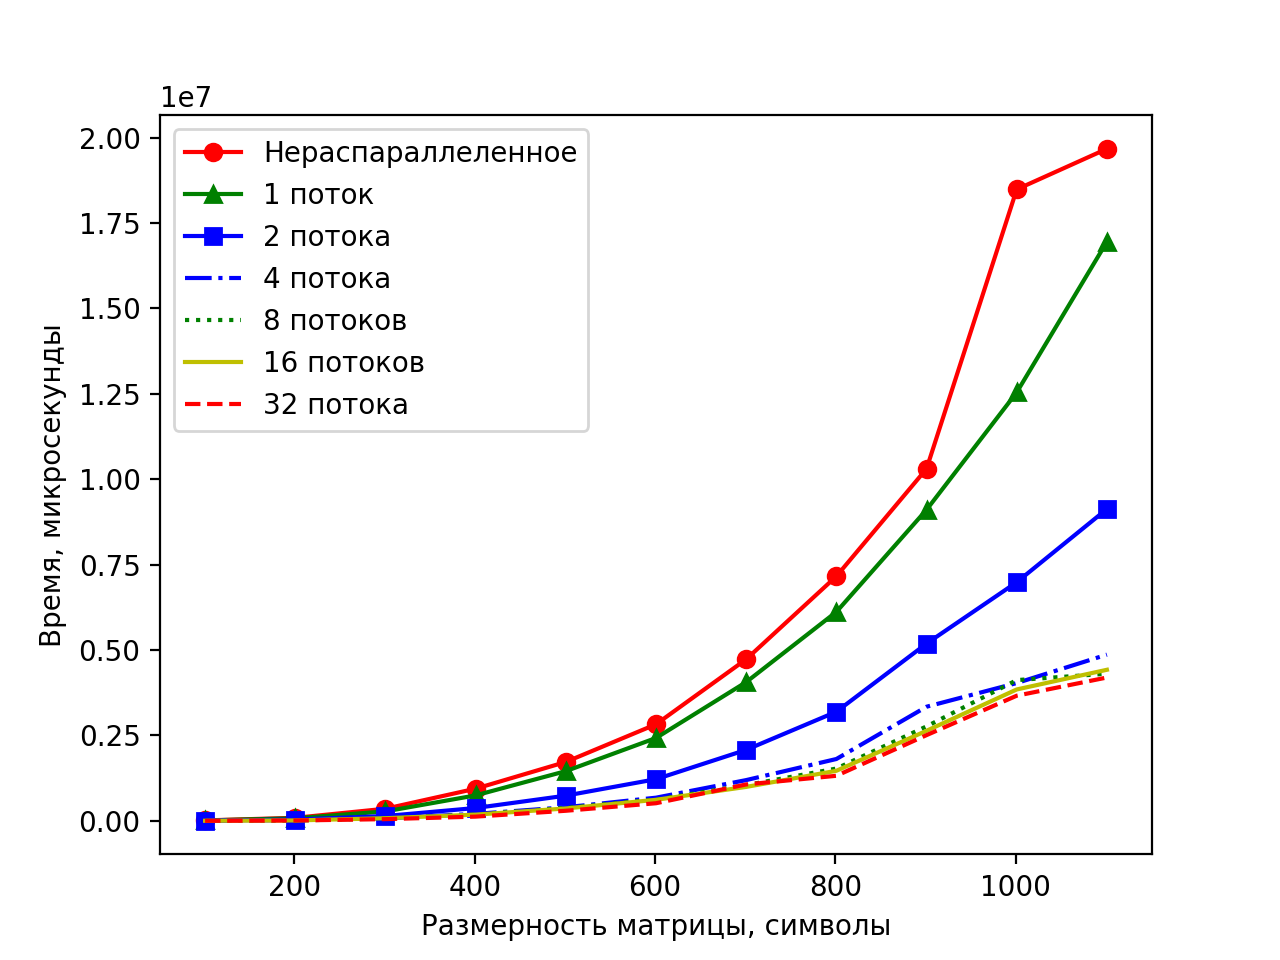
\includegraphics[scale = 1]{graph2} \\ Рис. 7 - Сравнение реализации алгоритмов нахождения произведения матриц при нечетных размерностях
	\end{center}
	
	\subsection{Выводы}
	\hfill
	
	Как мы видим из графиков предположения о более быстрой работе при использовании многопоточности подтвердились. Однако использование более 4 потоков не совсем оправдано. 
	
	Так, на графиках видим, что при использовании потоков с 4 до 32, скорость работы увеличивается незначительно, однако замеры времени не включают в себя создание потоков, соответственно, чем больше используется потоков, тем больше скорость работы. 
	
	В результате, оптимальным является использование 4 потоков. Скорость работы относительно многопоточного с 1 потоком, сокращается в 4 раза, а по сравнению с однопоточным в 4.5 раза. 
	
   	\newpage

        \anonsection{Заключение}
        
        \hfill
        
        В данной лабораторной работе было реализованы и пронализированы алгоритмы нахождения произведения матриц методом Винограда в многопоточном и однопоточном режимах. 
	
	\hfill
	
	Матрицы и матричное умножение активно применяется:
	\begin{enumerate}
		\item в сверточных слоях нейронных сетей для реализации прямого и обратного распространения сигнала
		\item в физике и математике для записи данных и их преобразования
		\item в компьютерной графике, для отображения изображений и их преобразований
		\item в психологии, для анализа результатов тестов
		\item в экономике, биологии, химии и других науках. 
	\end{enumerate}
	
	\hfill
	
	При сравнении данных алгоритмов пришли к следующим выводам:
	\begin{enumerate}
 		\item Что использование многопоточности значительно сокращает скорость работы программы.  
 		\item Однако не стоит создавать огромное количество потоков, ведь так вы проиграете по времени и по памяти на создании потоков. Оптималбное число потоков - 4. 
	\end{enumerate}
	
	\hfill
	
	В данной лабораторной работе выполнены следующие задачи. 
        \begin{enumerate} 
		\item Изучены алгоритмы умножения матриц: Винограда и его параллельная реализация. 
		\item Получены практические навыки реализации данных алгоритмов на одном из языков программирования. 
		\item Проведен сравнительный анализ алгоритмов по затрачиваемым ресурсам (зависимость времени от длины строки). 
		\item Экспериментально подтверждено различие в трудоемкости алгоритмов. 
	\end{enumerate}
        

 	\newpage

        \begin{thebibliography}{}
        		\bibitem{} [Электронный ресурс]. - Режим доступа: http://poivs.tsput.ru/ru/Math/Algebra/LinearAlgebra/Matrices (дата обращения: 22.10.2019)
		\bibitem{}  [Электронный ресурс]. - Режим доступа: https://habr.com/ru/post/359272/(дата обращения: 22.10.2019)
		\bibitem{}  [Электронный ресурс]. - Режим доступа: https://urok.1sept.ru/статьи/637896/(дата обращения: 22.10.2019)
		\bibitem{}  [Электронный ресурс]. - Режим доступа: http://we.easyelectronics.ru/Theory/cifrovye-rekursivnye-filtry-chast-1.html(дата обращения: 22.10.2019)
		\bibitem{}  [Электронный ресурс]. - Режим доступа: http://window.edu.ru/resource/898/72898/files/stup559.pdf(дата обращения: 22.10.2019)
		\bibitem{}  [Электронный ресурс]. - Режим доступа: http://vekkv.ru/holotropnoe-dyhanie-transpersonalnaya-psihologiya/1859/(дата обращения: 22.10.2019)
		\bibitem{} [Электронный ресурс]. - Режим доступа:  https://www.eduherald.ru/ru/article/view?id=14118(дата обращения: 22.10.2019)
		\bibitem{}  [Электронный ресурс]. - Режим доступа: https://cyberleninka.ru/article/n/matrichnyy-printsip-v-biologii-progiloe-nastoyaschee-buduschee(дата обращения: 22.10.2019)
		\bibitem{}  [Электронный ресурс]. - Режим доступа: http://www.chemicals-el.ru/chemicals-2400-1.html(дата обращения: 22.10.2019)
		\bibitem{} [Электронный ресурс] - Режим доступа: https://habr.com/ru/post/39543/ (дата обращения: 22.10.2019)
		\bibitem{} [Электронный ресурс] - Режим доступа: https://xakep.ru/2013/10/25/polythread-soft/ (дата обращения: 22.10.2019)
	\end{thebibliography} 

\end{document}
